\documentclass{standalone}
\usepackage[T1]{fontenc}
\usepackage[latin2]{inputenc}
\usepackage[english]{babel}
\usepackage{tikz}
\usetikzlibrary{calc,through,backgrounds,positioning,fit}
\usetikzlibrary{shapes,arrows,shadows}
\tikzstyle{stt}=[shape=circle, draw, minimum height=6mm]
\begin{document}
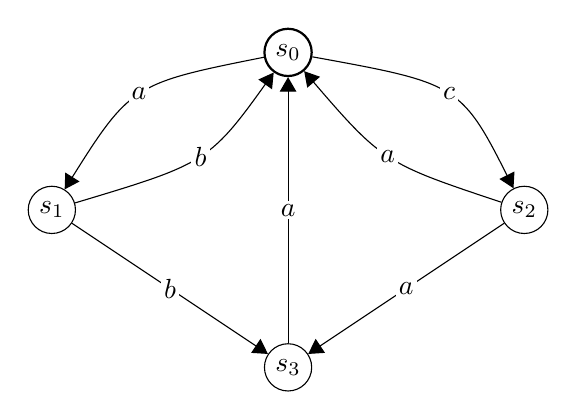
\begin{tikzpicture}[scale=1,inner sep=0.4mm]
\node (s0) [stt,thick] at (0,2) {$s_0$};
\node (s1) [stt] at (-3,0) {$s_1$};
\node (s2) [stt] at (3,0) {$s_2$};
\node (s3) [stt] at (0,-2) {$s_3$};
 
\draw[-triangle 60] (s0) .. node [fill=white] {$c$} controls (2.2,1.6) and (2.2,1.6)  .. (s2);
\draw[-triangle 60] (s2) .. node [fill=white] {$a$} controls (1.2,0.6) and (1.2,0.6)  .. (s0);

\draw[-triangle 60] (s1) .. node [fill=white] {$b$} controls (-1,0.6) and (-1,0.6)  .. (s0);
\draw[-triangle 60] (s0) .. node [fill=white] {$a$} controls (-2,1.6) and (-2,1.6)  .. (s1);


\draw[-triangle 60] (s2) -- node [fill=white] {$a$} (s3);
\draw[-triangle 60] (s1) -- node [fill=white] {$b$} (s3);
\draw[-triangle 60] (s3) -- node [fill=white] {$a$} (s0);
%\draw[-triangle 60] (s3) -- node [fill=white] {$a$} (s4);
%\draw[-triangle 60] (s1) .. node [fill=white] {$a$} controls (-3,-2) and (-1,-2.7)  .. (s4);
%\draw[-triangle 60] (s4) .. node [fill=white] {$c$} controls (0,-1.5) and (-2,-1) .. (s1);

 
\end{tikzpicture}
\end{document}